\documentclass[aspectratio=149, xcolor=table]{beamer}
\usetheme{Montpellier}
\usefonttheme{serif}
\usecolortheme{dove}
\useinnertheme{rounded}
\setbeamersize{text margin left=5mm,text margin right=10mm}
\usefonttheme{serif}
\usepackage{graphicx}
\usepackage{babel}
\usepackage[utf8]{inputenc}
\usepackage{tabularx}
\usepackage{tikz}
\usepackage[absolute,overlay]{textpos} 
\usepackage{xcolor}
\usepackage{multicol}
\definecolor{myGreen}{RGB}{54, 114, 89}
\definecolor{unipd}{RGB}{155, 0, 20}
\definecolor{sbj1}{HTML}{77AC30}
\definecolor{sbj2}{HTML}{EDB120}
\definecolor{sbj3}{HTML}{0072BD}
\definecolor{sbj4}{HTML}{1F78B4}
\definecolor{sbj5}{HTML}{33A02C}
\definecolor{sbj6}{HTML}{E31A1C}
% Per il tema Montpellier
%\setbeamercolor{separation line}{bg=myGreen!20}
\setbeamercolor{separation line}{bg=black!20}
%\setbeamercolor{title in head/foot}{bg=white, fg=myGreen}
\setbeamercolor{title in head/foot}{bg=white, fg=black}
%\setbeamercolor{section in head/foot}{bg=white, fg=myGreen}
%\setbeamercolor{subsection in head/foot}{bg=white, fg=myGreen}
%\setbeamercolor{background canvas}{bg=white}
%\setbeamercolor{title}{fg=myGreen}
%\setbeamercolor{item}{fg =myGreen}
%\setbeamercolor{frametitle}{fg = myGreen}
%\setbeamercolor{section in toc}{fg=myGreen!80}
%\setbeamercolor{subsection in toc}{fg=black}
\setbeamerfont{section in toc}{series=\bfseries,size=\normalsize}
\setbeamerfont{frametitle}{series=\bfseries}
%\setbeamerfont{title}{family=\scshape}
%\setbeamercolor{frametitle}{fg=unipd}
%\setbeamercolor{section in head/foot}{bg=unipd, fg=white}
%\setbeamercolor{subsection in head/foot}{fg=unipd}
%\setbeamercolor{author in head/foot}{bg=unipd, fg=white}
%\setbeamercolor{title in head/foot}{fg=unipd}
%\setbeamercolor{date in head/foot}{fg=unipd}

% definisce gli elementi da mettere sopra la figura 
% rectangles on figures 
\newcommand{\imagenode}[2][1]% [scale], filename
{   \node[above right,inner sep=0] (myimage) {\includegraphics[scale=#1]{#2}};
	\path (myimage.north east);
	\pgfgetlastxy{\myimagex}{\myimagey}
	\pgfmathsetmacro{\myimagewidth}{\myimagex/28.453}
	\pgfmathsetmacro{\myimageheight}{\myimagey/28.453}
}
\newcommand{\imagegrid}[4][help lines]% [options], steps, font, precision
{   \pgfkeys{/pgf/number format/.cd,fixed,precision=#4}
	\foreach \x in {0,...,#2}
	{   \draw[#1] (\x/#2*\myimagewidth,\myimageheight) -- (\x/#2*\myimagewidth,0) node[below] {#3\pgfmathparse{\x/#2}\pgfmathprintnumber{\pgfmathresult}};
		\draw[#1] (\myimagewidth,\x/#2*\myimageheight) -- (0,\x/#2*\myimageheight) node[left] {#3\pgfmathparse{\x/#2}\pgfmathprintnumber{\pgfmathresult}};
	}
}

\newcommand{\highlightbox}[8][densely dashed,thick]% [options], left, low, right, up, node options, node text, overlay spec
{   \only<#8>{\draw[#1] (#2*\myimagewidth, #3*\myimageheight) rectangle node[#6] {#7} (#4*\myimagewidth, #5*\myimageheight);}
}

\newcommand{\highlighttext}[8][densely dashed,thick]% [options], left, low, right, up, node options, node text, overlay spec
{   \only<#8>{\path[#1] (#2*\myimagewidth, #3*\myimageheight) rectangle node[#6] {#7} (#4*\myimagewidth, #5*\myimageheight);}
}

% tikz per la cfa 

\usetikzlibrary{shapes.geometric, arrows}
\tikzstyle{latent} = [ellipse, minimum width=2.5cm, minimum height=2cm,text centered, draw=black]
\tikzstyle{item} = [rectangle, rounded corners, minimum width=0.5cm, minimum height=1cm, text width =1.5cm, text centered, draw=black]
\tikzstyle{arrow} = [thick,->,>=stealth]

% allegedly, il codice che viene dopo permette di cambiare colore alle celle 

\makeatletter
\def\rowcolor{\noalign{\ifnum0=`}\fi\bmr@rowcolor}
\newcommand<>{\bmr@rowcolor}{%
	\alt#1%
	{\global\let\CT@do@color\CT@@do@color\@ifnextchar[\CT@rowa\CT@rowb}% 
	{\ifnum0=`{\fi}\@gooble@rowcolor}% 
}

\newcommand{\@gooble@rowcolor}[2][]{\@gooble@rowcolor@}
\newcommand{\@gooble@rowcolor@}[1][]{\@gooble@rowcolor@@}
\newcommand{\@gooble@rowcolor@@}[1][]{\ignorespaces}
\makeatother



\makeatletter
\def\cellcolor{{\ifnum0=`}\fi\bmr@cellcolor}
\newcommand<>{\bmr@cellcolor}{%
	\alt#1%
	{\global\let\CT@do@color\CT@@do@color\@ifnextchar[\CT@rowa\CT@rowb}% 
	{\ifnum0=`{\fi}\@gooble@cellcolor}% 
}

\newcommand{\@gooble@cellcolor}[2][]{\@gooble@cellcolor@}
\newcommand{\@gooble@cellcolor@}[1][]{\@gooble@cellcolor@@}
\newcommand{\@gooble@cellcolor@@}[1][]{\ignorespaces}
\makeatother

\DeclareMathOperator*{\argmax}{arg\,max}
\DeclareMathOperator*{\argmin}{arg\,min}

\AtBeginSection[]
{
	\begin{frame}
		\tableofcontents[currentsection, currentsubsection]
	\end{frame}
}

\AtBeginSubsection[]
{
	\begin{frame}
		\tableofcontents[currentsection, currentsubsection]
	\end{frame}
}


\title[ILA]{It's how you use the items that counts: \\ An intelligent procedure for item selection in Item Response Theory}
\author{Ottavia M. Epifiania\textsuperscript{1}, Pasquale Anselmi\textsuperscript{3}, Egidio Robusto\textsuperscript{3}}

\institute [UniPd] {
	%\includegraphics[width=10mm]{unipd.png}\\ 
	\textsuperscript{1} Psychology and Cognitive Science Department, University of Trento, Italy \\
	\textsuperscript{2} Psicostat, University of Padova, Italy \\
	\textsuperscript{3} Department of Philosophy, Sociology, Education, and Applied Pscyhology,	University of Padova, Italy}

\date [ASA2024] {%\vspace{0.6cm}\\
	Convegno ASA 2024\\ Contributed session: Developing, administering and refining measurement instruments in Social Sciences \\ \vspace{3mm}
	19 Settembre 2024}
\begin{document}
\begin{frame}[plain]
    \maketitle
\end{frame}

\section{Aim}
\begin{frame}
	New Item Response Theory-based algorithm for the development of informative short test forms
\end{frame}

\section{Item Response Theory and Information Functions}
\subsection{2-Parameter Logistic Model}

\begin{frame}
\centering

	
	\centering
	\onslide<1>
	\vspace*{1mm}
	
	$P(x_{pi} = 1|\theta_p, b_i, a_i) = \frac{\exp[a_i(\theta_p - b_i)]}{1 + \exp[a_i(\theta_p - b_i)]}$
	
	\vspace{1.5mm}
	\centering
	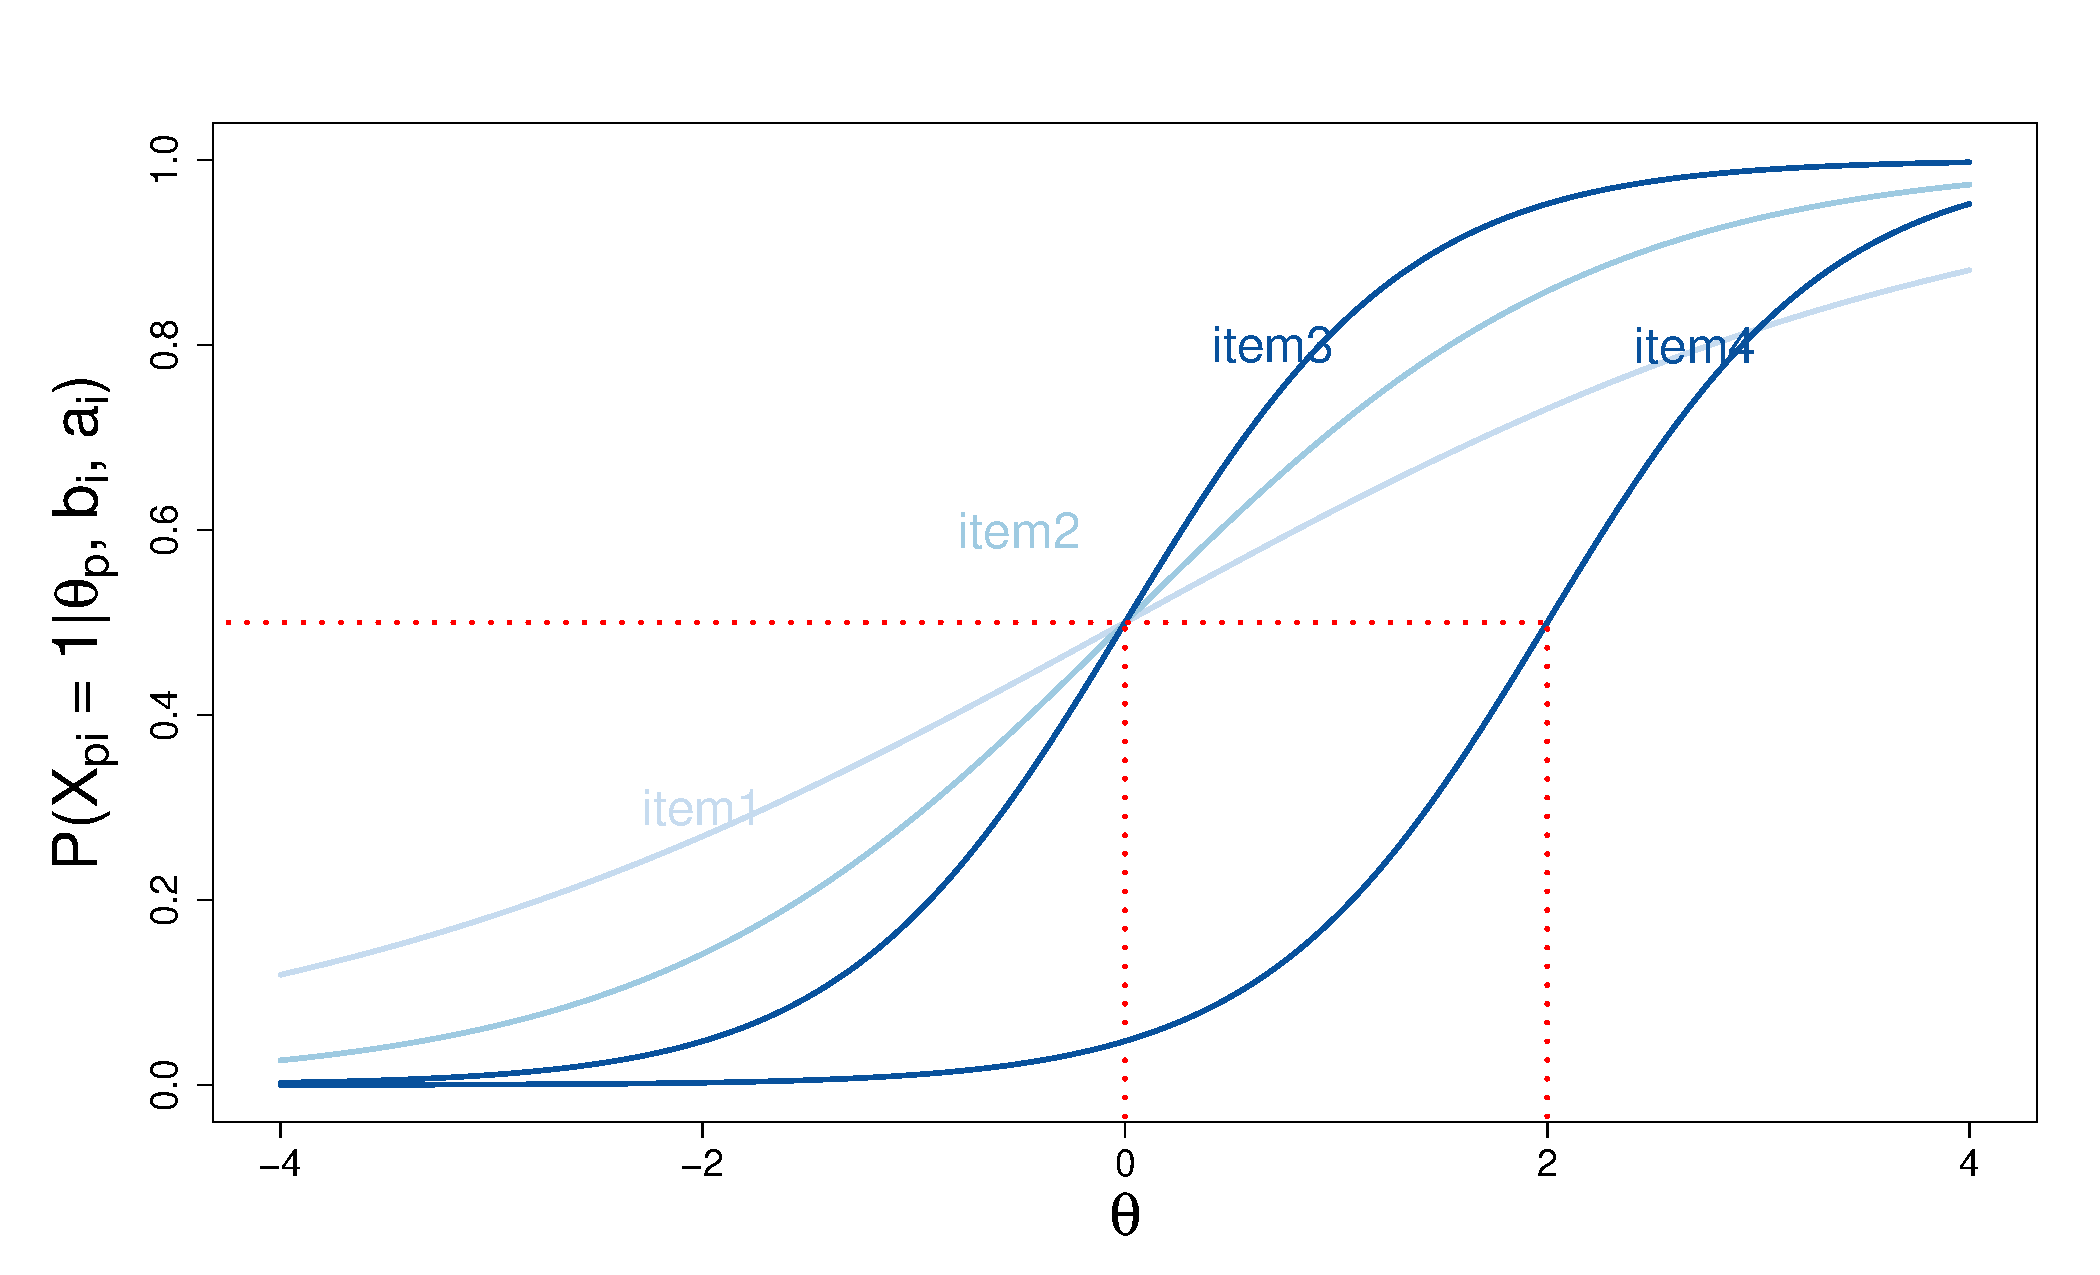
\includegraphics[width=.70\linewidth]{img/ICC-2pl.pdf}
	
	
\end{frame}

\subsection{Item and Test Information Functions}
\begin{frame}
	
	\begin{columns}[T]
	\begin{column}{.5\linewidth}
		\centering
		Item Information Function (IIF): \\	$I_i(\theta) = a_i^2P_i(\theta, b_i, a_i)[1-P_i(\theta, b_i, a_i)]$
		
		\centering
		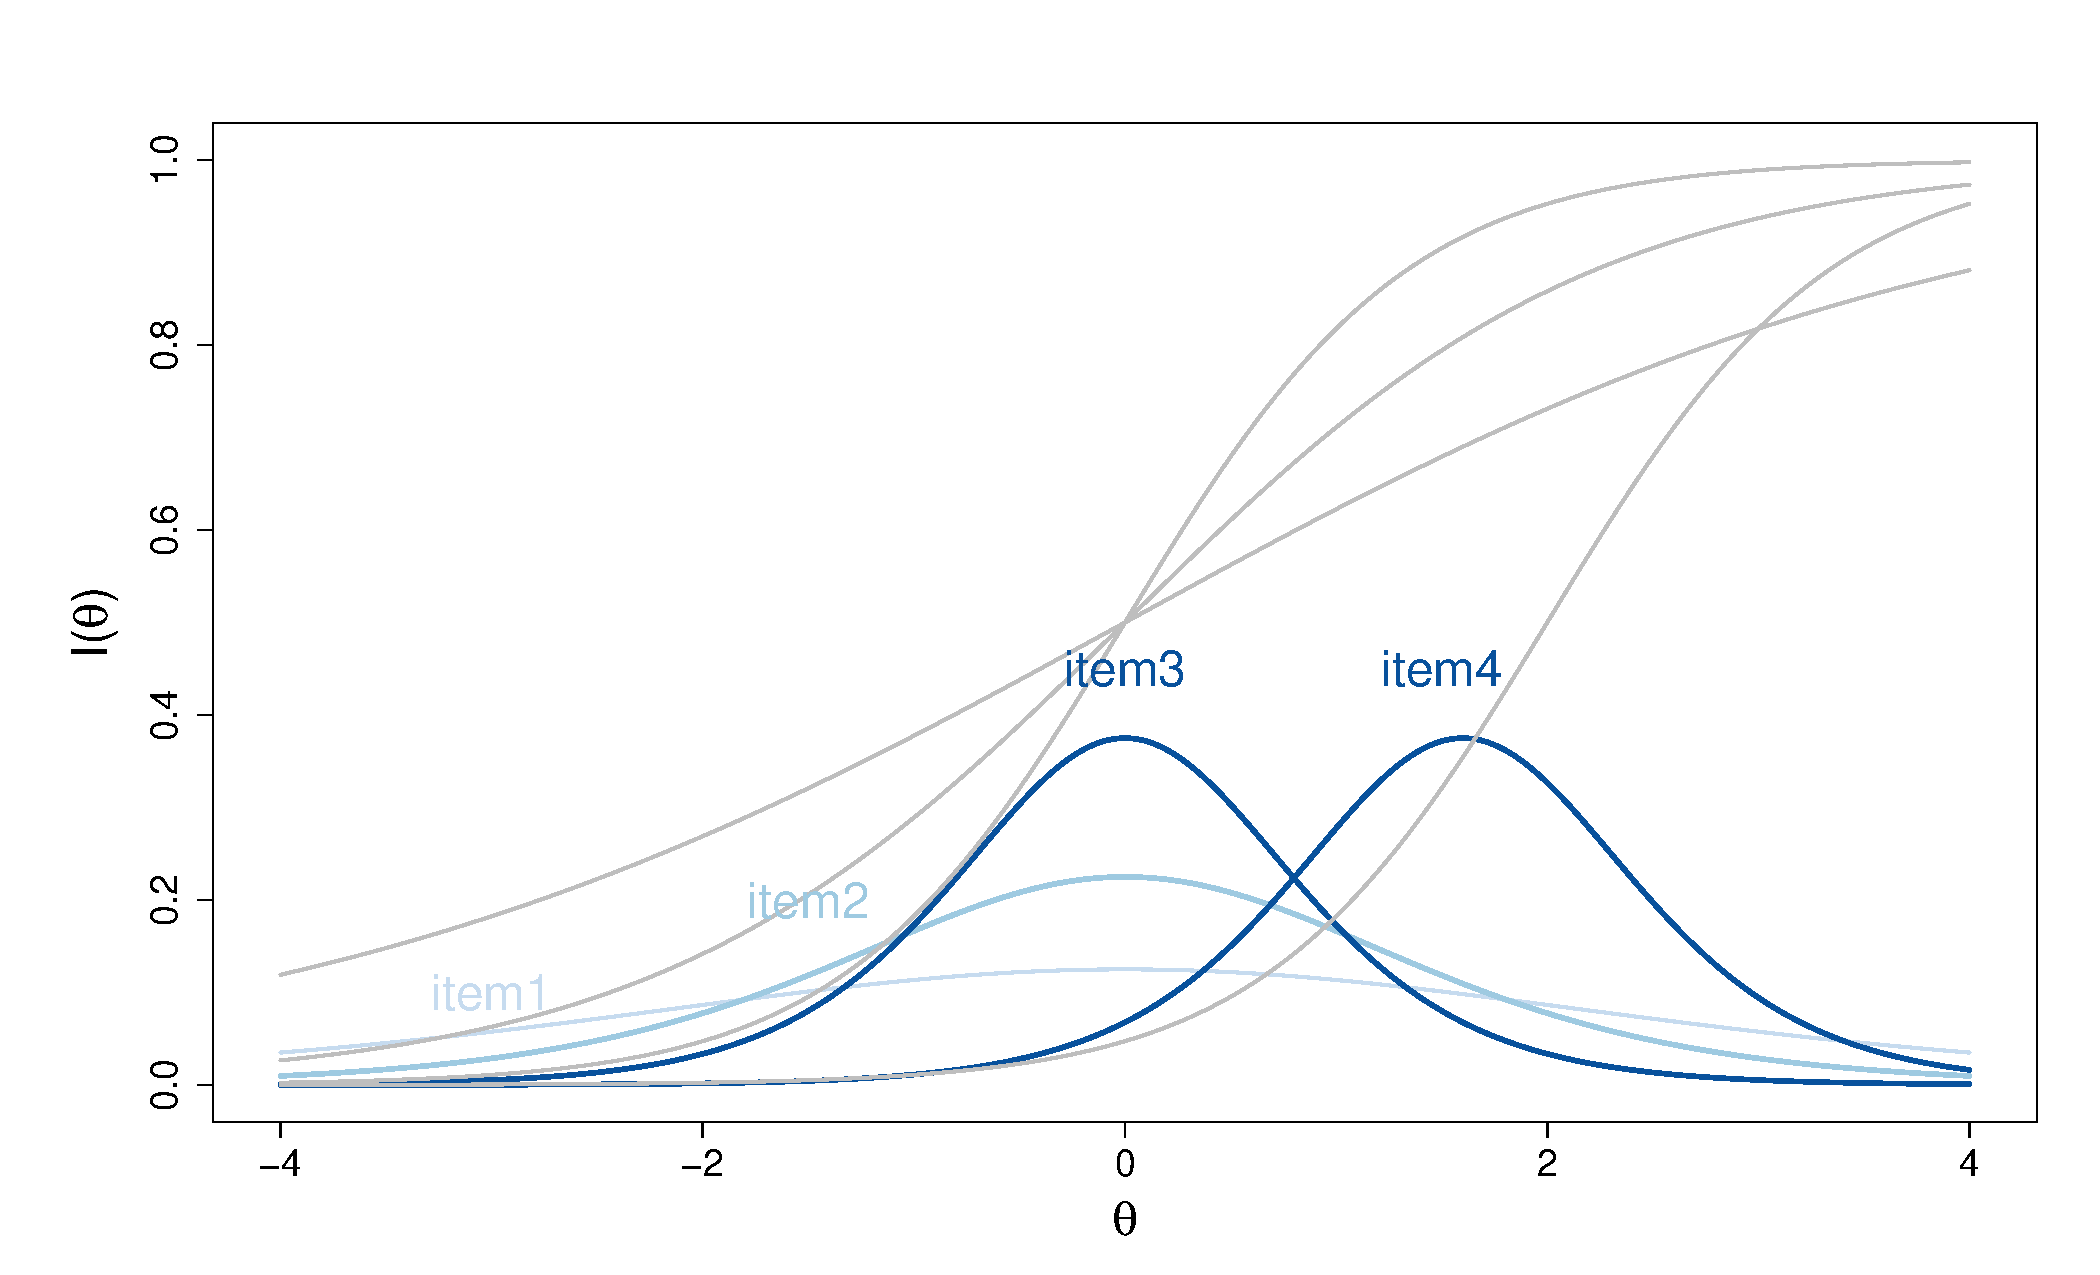
\includegraphics[width=\linewidth]{img/IIF-2pl.pdf}
		
	\end{column}
	\begin{column}{.5\linewidth}
		\centering
		Test Information Function (TIF):	\\	$I(\theta) =  \sum_{i = 1}^{I} I_i(\theta)$
	
	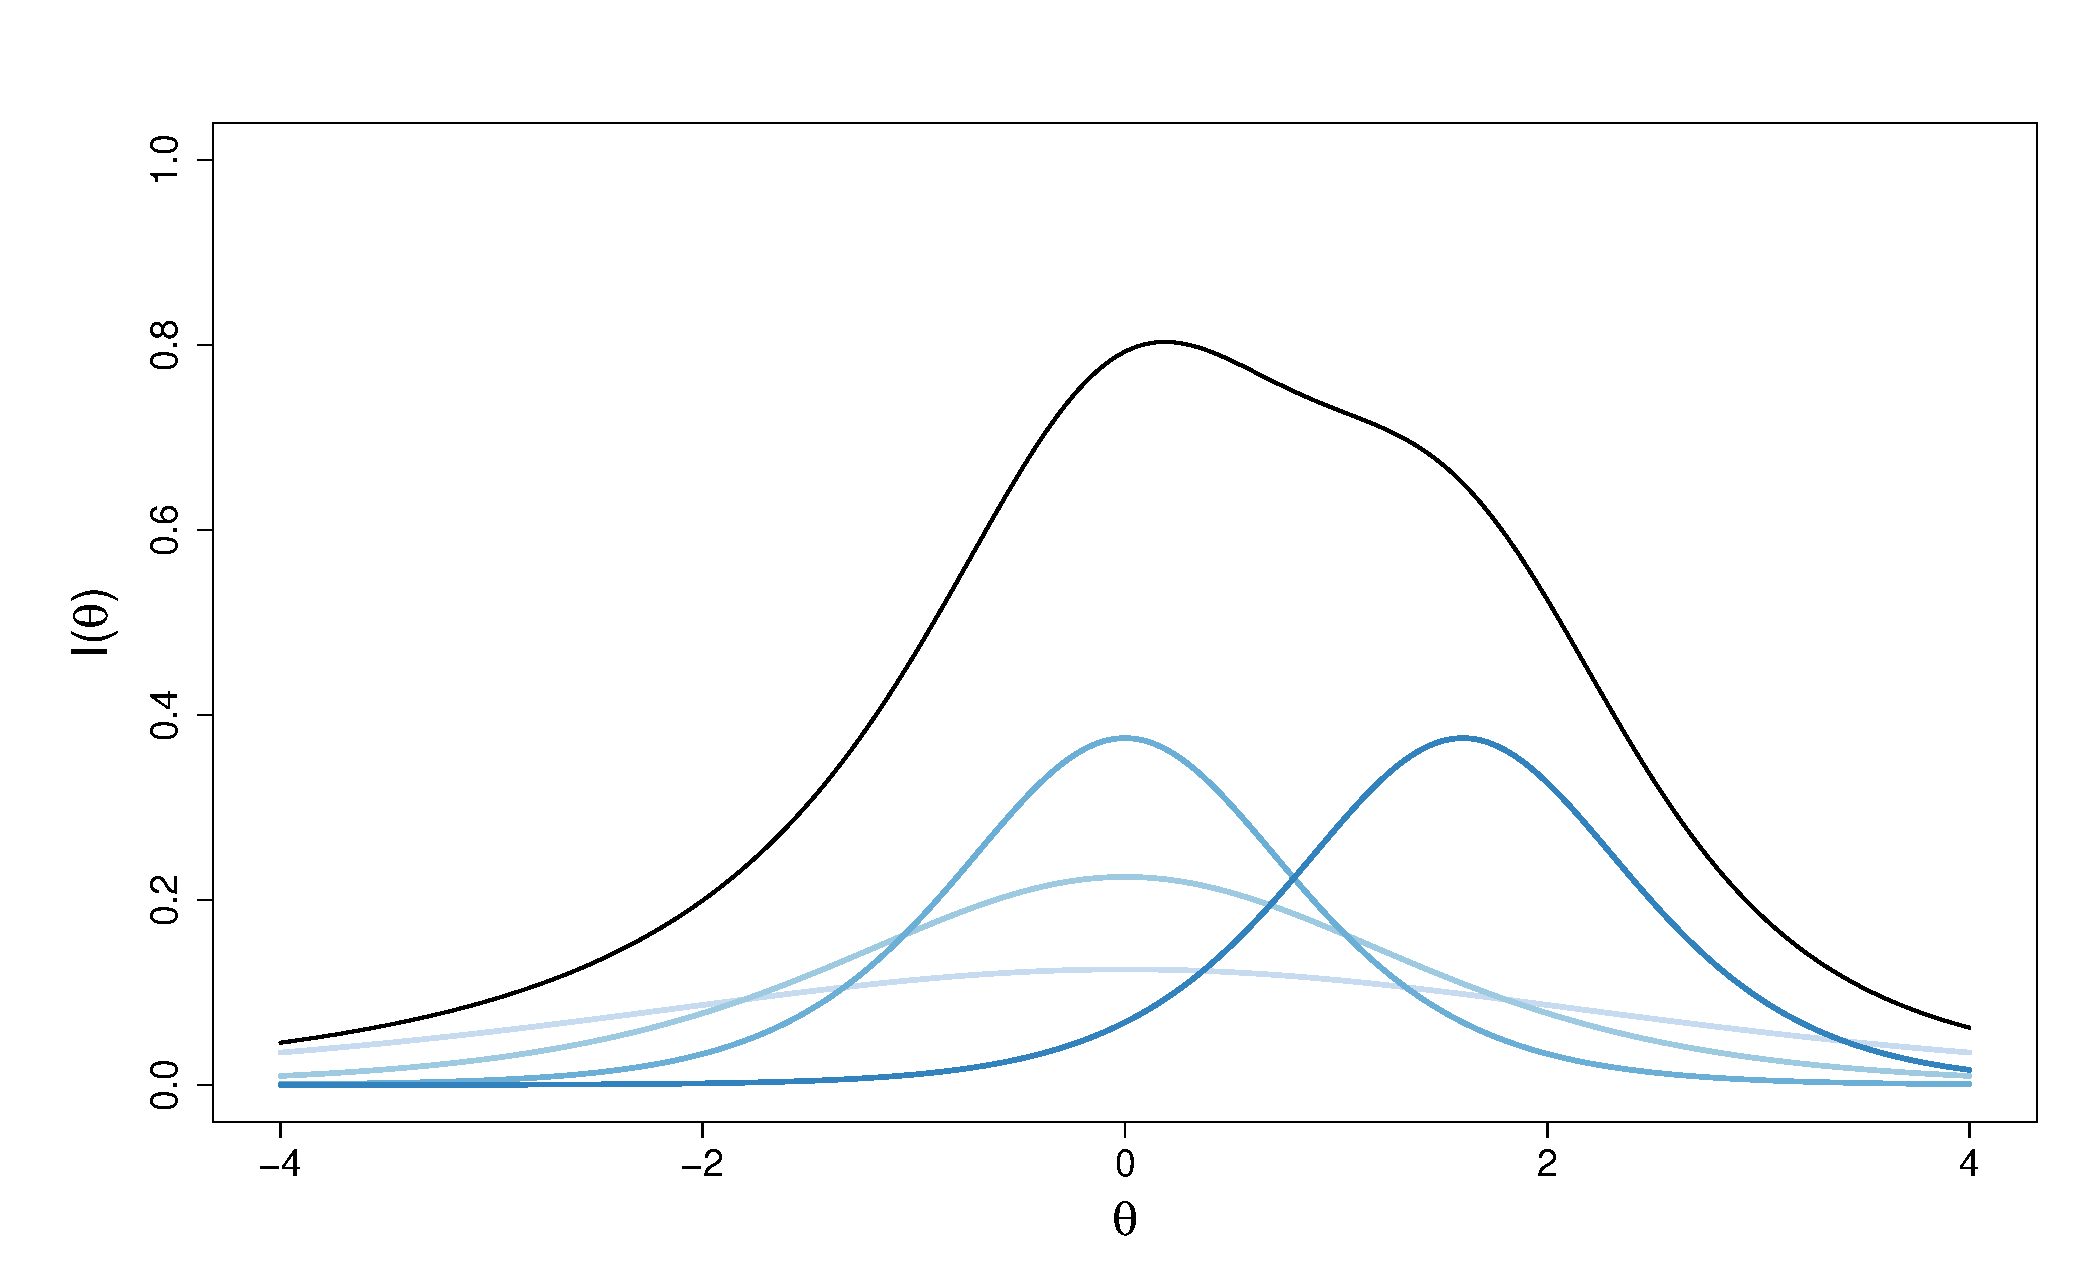
\includegraphics[width=\linewidth]{img/TIF-2pl.pdf}
	
	\end{column}
	\end{columns}
		
\end{frame}

\section{Item Selection Procedures}



\subsection{Item Locating Algorithm -- ILA}
\begin{frame}
	
$Q^k$: vector of the item indexes selected for inclusion in the STF up to iteration $k$ ($Q^0 = \emptyset$)
	
$\mathit{TIF}^*$: TIF target 

%$TIF^k = \frac{\sum_{i\in Q^k} IIF_i}{||Q^k||}$, where $||Q^k||$ denotes the cardinality of $Q^k$, 
$TIF^0 = 0$ 

\color{blue} Termination criterion: $|TIF^* - TIF^k| \leq |TIF^* - TIF^{k-1}|$ \normalcolor

Iterate: 
	\begin{enumerate}
		%\item  $\Delta_{TIF}^k = |TIF^* - TIF^k|$ %Since at the beginning no items are selected for inclusion in the STF, $Q = \emptyset$ and $||Q|| =0$, so $\Delta_{TIF} = |TIF^* - 0|$. 
		
		\item  %A $\theta_{target}$ is determined as the $\theta$ level for which the absolute distance between the $\mathit{TIF}^*$ and $\mathit{TIF}_{TE}$ is maximum, 
		$\theta_{target} =\argmax{|TIF^* - TIF^{k-1}|}$ %At the first iteration, it will be the $\theta$ level with the highest information function. 
		
		\item  %The index of the first item to be included in $Q$ is the index of the item whose location is closest to the $\theta_{target}$, 
	\color{blue}	$Q^{k} = Q^{k-1} \cup \argmin_{i \in \{1, \ldots, N\}\setminus Q^{k-1}} |\theta_{target} -b_i|$ \normalcolor
		
		\item  $TIF^{k} = \frac{\sum_{i\in Q^k} IIF_i}{||Q^k||}$
		
		\item $k =  k +1$ 
		
	\end{enumerate}
\end{frame}

\subsection{Brute Force Procedure}
\begin{frame}
	$N$: Number of items in the item bank 
	
	$L = N-1$: Maximum length of the STFs that can developed from the item bank 
	
	$\binom{N}{l}$: number of STFs resulting from the combination of the $l = \{1, \ldots L\}$ items 
	
 The algorithm iterates the following steps until the termination criterion is reached: 
 
 \begin{enumerate}
 	\item $\overline{\mathit{TIF}}$ for each STF of length $l$
 	\item $\Delta_{TIF} = TIF^* - \overline{\mathit{TIF}}$
 	\item $\overline{\Delta}_{TIF}$
 \end{enumerate}
	
	The best STF is the one with the lowest value of $\overline{\Delta}_{TIF}$, that is the one that presents the lowest absolute distance from the TIF target.
\end{frame}

\section{Simulation Study}

\subsection{Simulation design}
\begin{frame}
	
100 iterations: 

\begin{enumerate}
	\item  Generate an item bank of $N = 6$ items: 
	\begin{itemize}
		\item Difficulty parameters: $\mathcal{U}(-3, 3)$
		\item Discrimination parameters:  $\mathcal{U}(.90, 2.0)$
	\end{itemize} 
	
	\item  Generate $TIF^*$ by randomly selecting items from the item bank (Mean number of items $= 3.34 \pm 1.13$). The parameters of the selected items are modified according to values drawn from uniform distributions $\mathcal{U}(-0.20, 0.20)$. 
	
	
	\item  Considering the $TIF^*$ at Step 2 and the item parameters at Step 1:
	\begin{itemize}
		\item ILA $\rightarrow$ Forwardly searches for the best item selection to recover the $TIF^*$
		\item BFP $\rightarrow$ tries every possible item combination to find the STF best able to recover $TIF^*$ $N=6$ items, $L = 5$ and $\binom{6}{1} + \binom{6}{2} + \binom{6}{3} + \binom{6}{4} + \binom{6}{5} =  62$ STFs are developed and compared.
	\end{itemize}
	
\end{enumerate}
\end{frame}

\subsection{Comparison}

\begin{frame}
	\begin{itemize}
		\item $||Q_{\text{BFP}}|| - ||Q_{\text{ILA}}||$ 
		\item Percentile rank of the distance between the STF selected by BFP and that selected by ILA
	\end{itemize}
\end{frame}


\subsection{Results}



\begin{frame}
	57\% $||Q_{\text{BFP}}|| - ||Q_{\text{ILA}}|| = 0$  $\rightarrow$ 72\% same item selection
	\begin{figure}
		\centering
		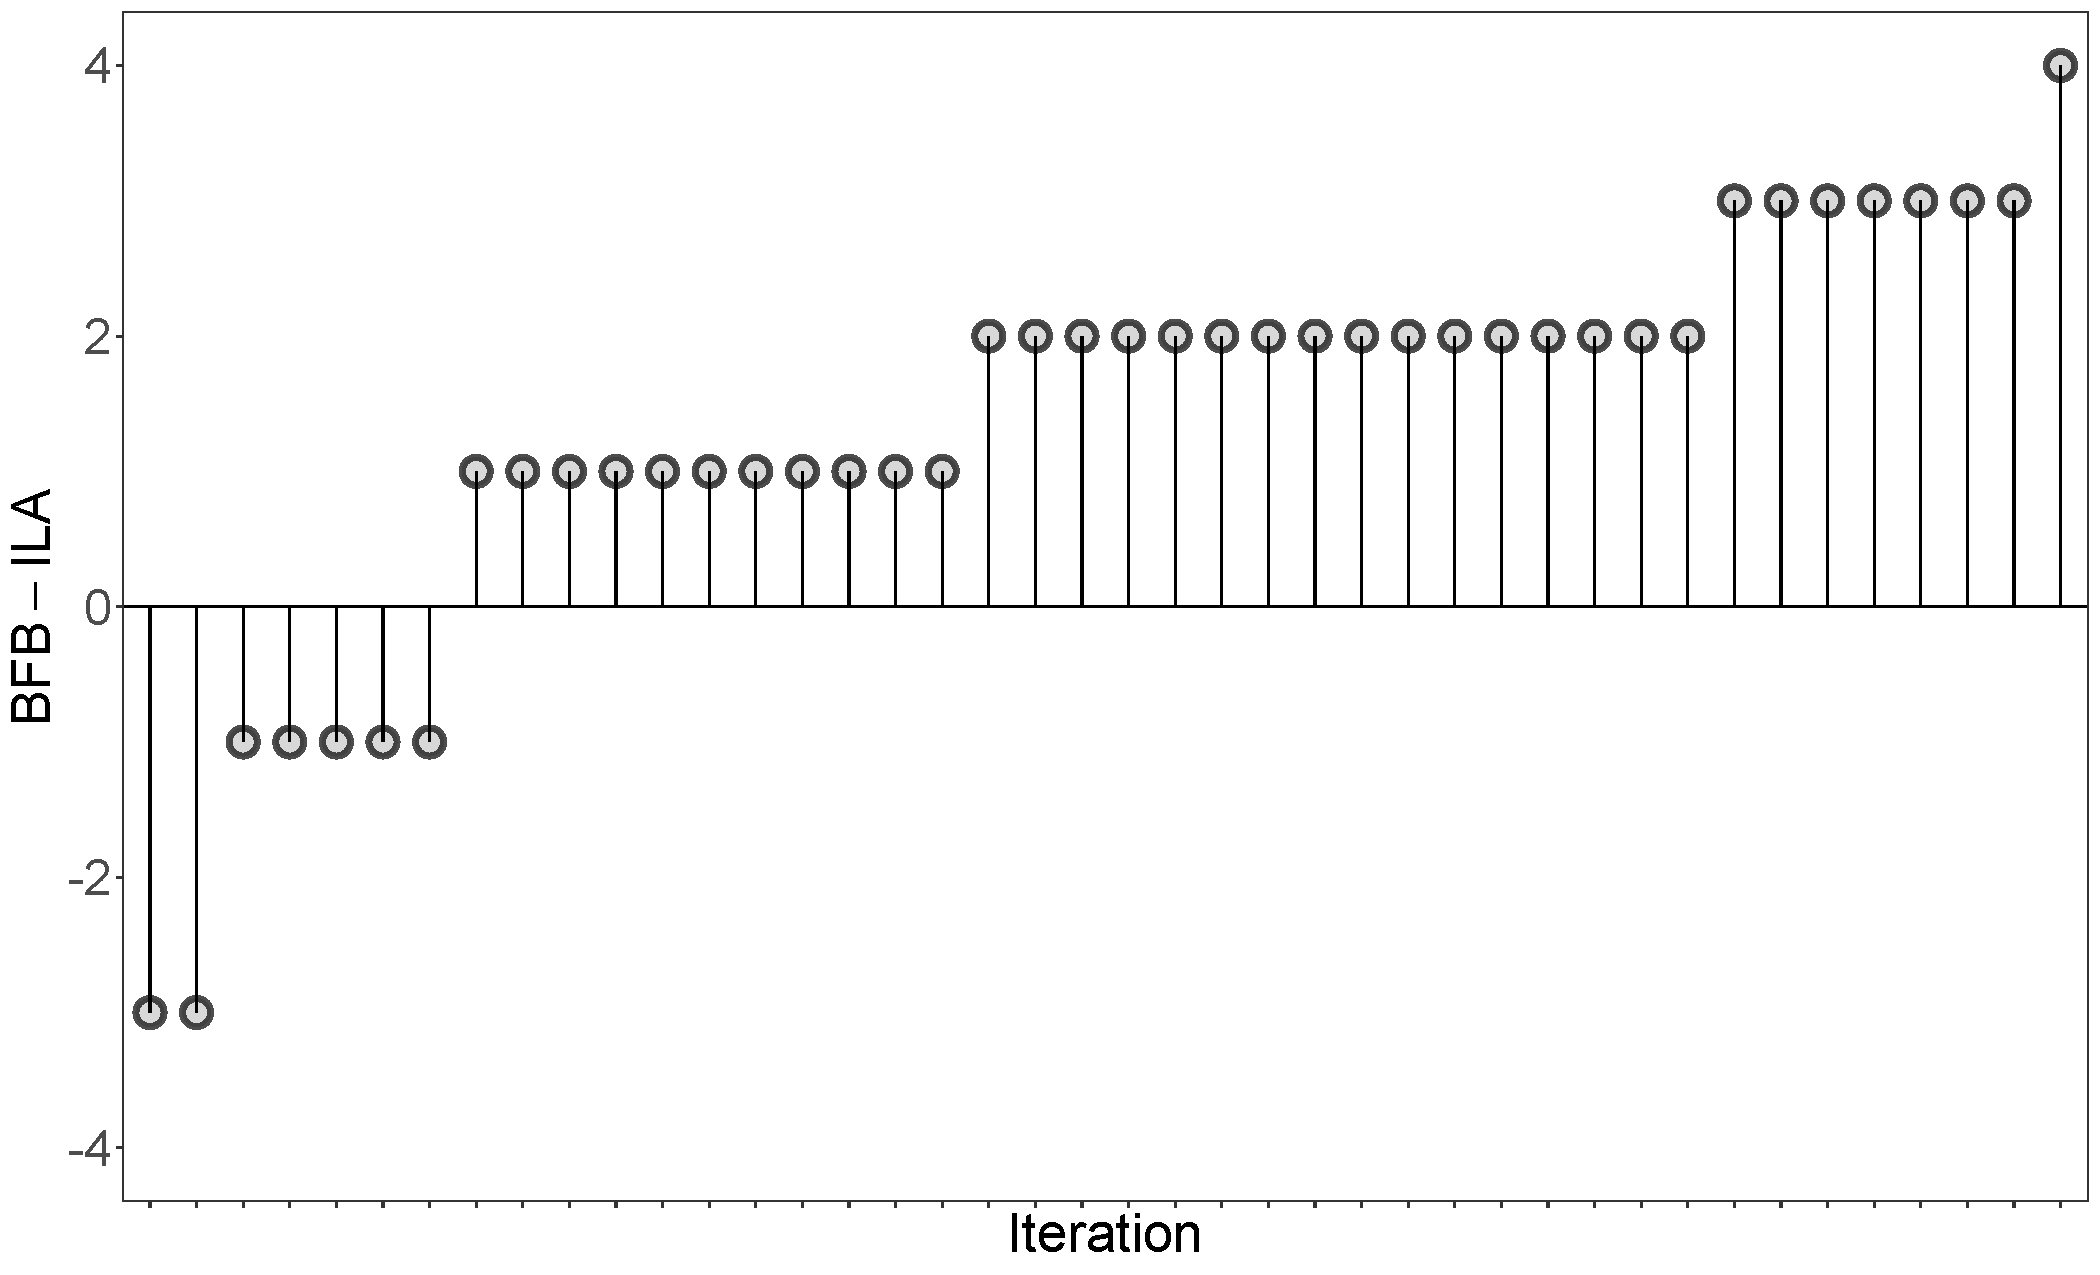
\includegraphics[width=.80\linewidth]{img/bfp-ila}
		\caption{43\% $||Q_{\text{BFP}}|| - ||Q_{\text{ILA}}|| \neq 0$ }
	\end{figure}
\end{frame}

\begin{frame}
	\begin{figure}
		\centering
		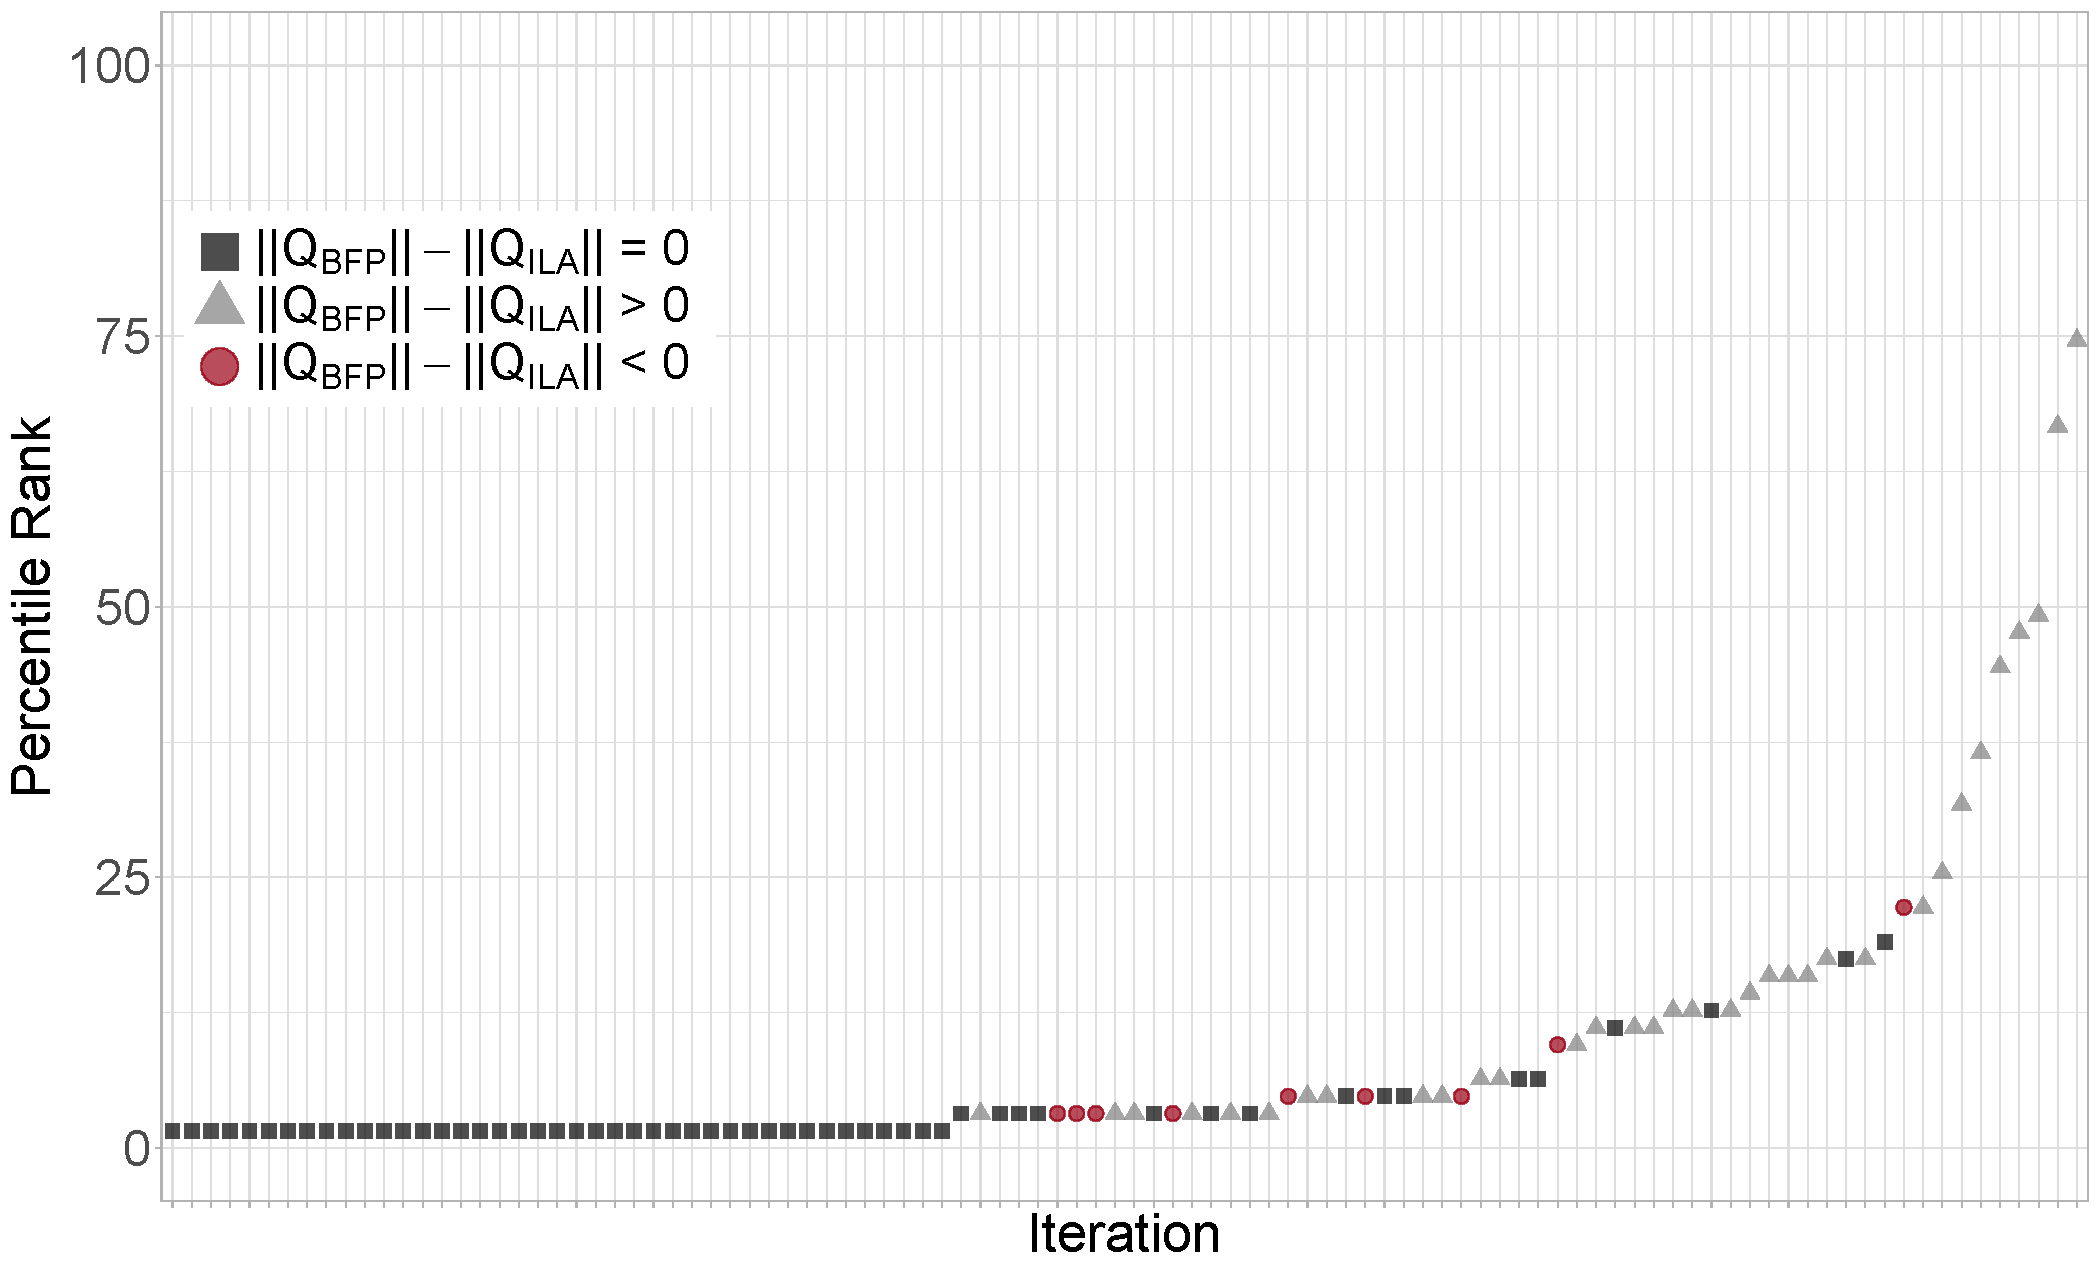
\includegraphics[width=\linewidth]{img/rp}
	\end{figure}
\end{frame}


\begin{frame}
	
	\begin{columns}[T]
	\begin{column}{.50\linewidth}

	\centering
		\footnotesize{$||Q_{\text{BFP}}|| = ||Q_{\text{ILA}}||$, $Q_{\text{BFP}} \neq Q_{\text{ILA}}$}
	
	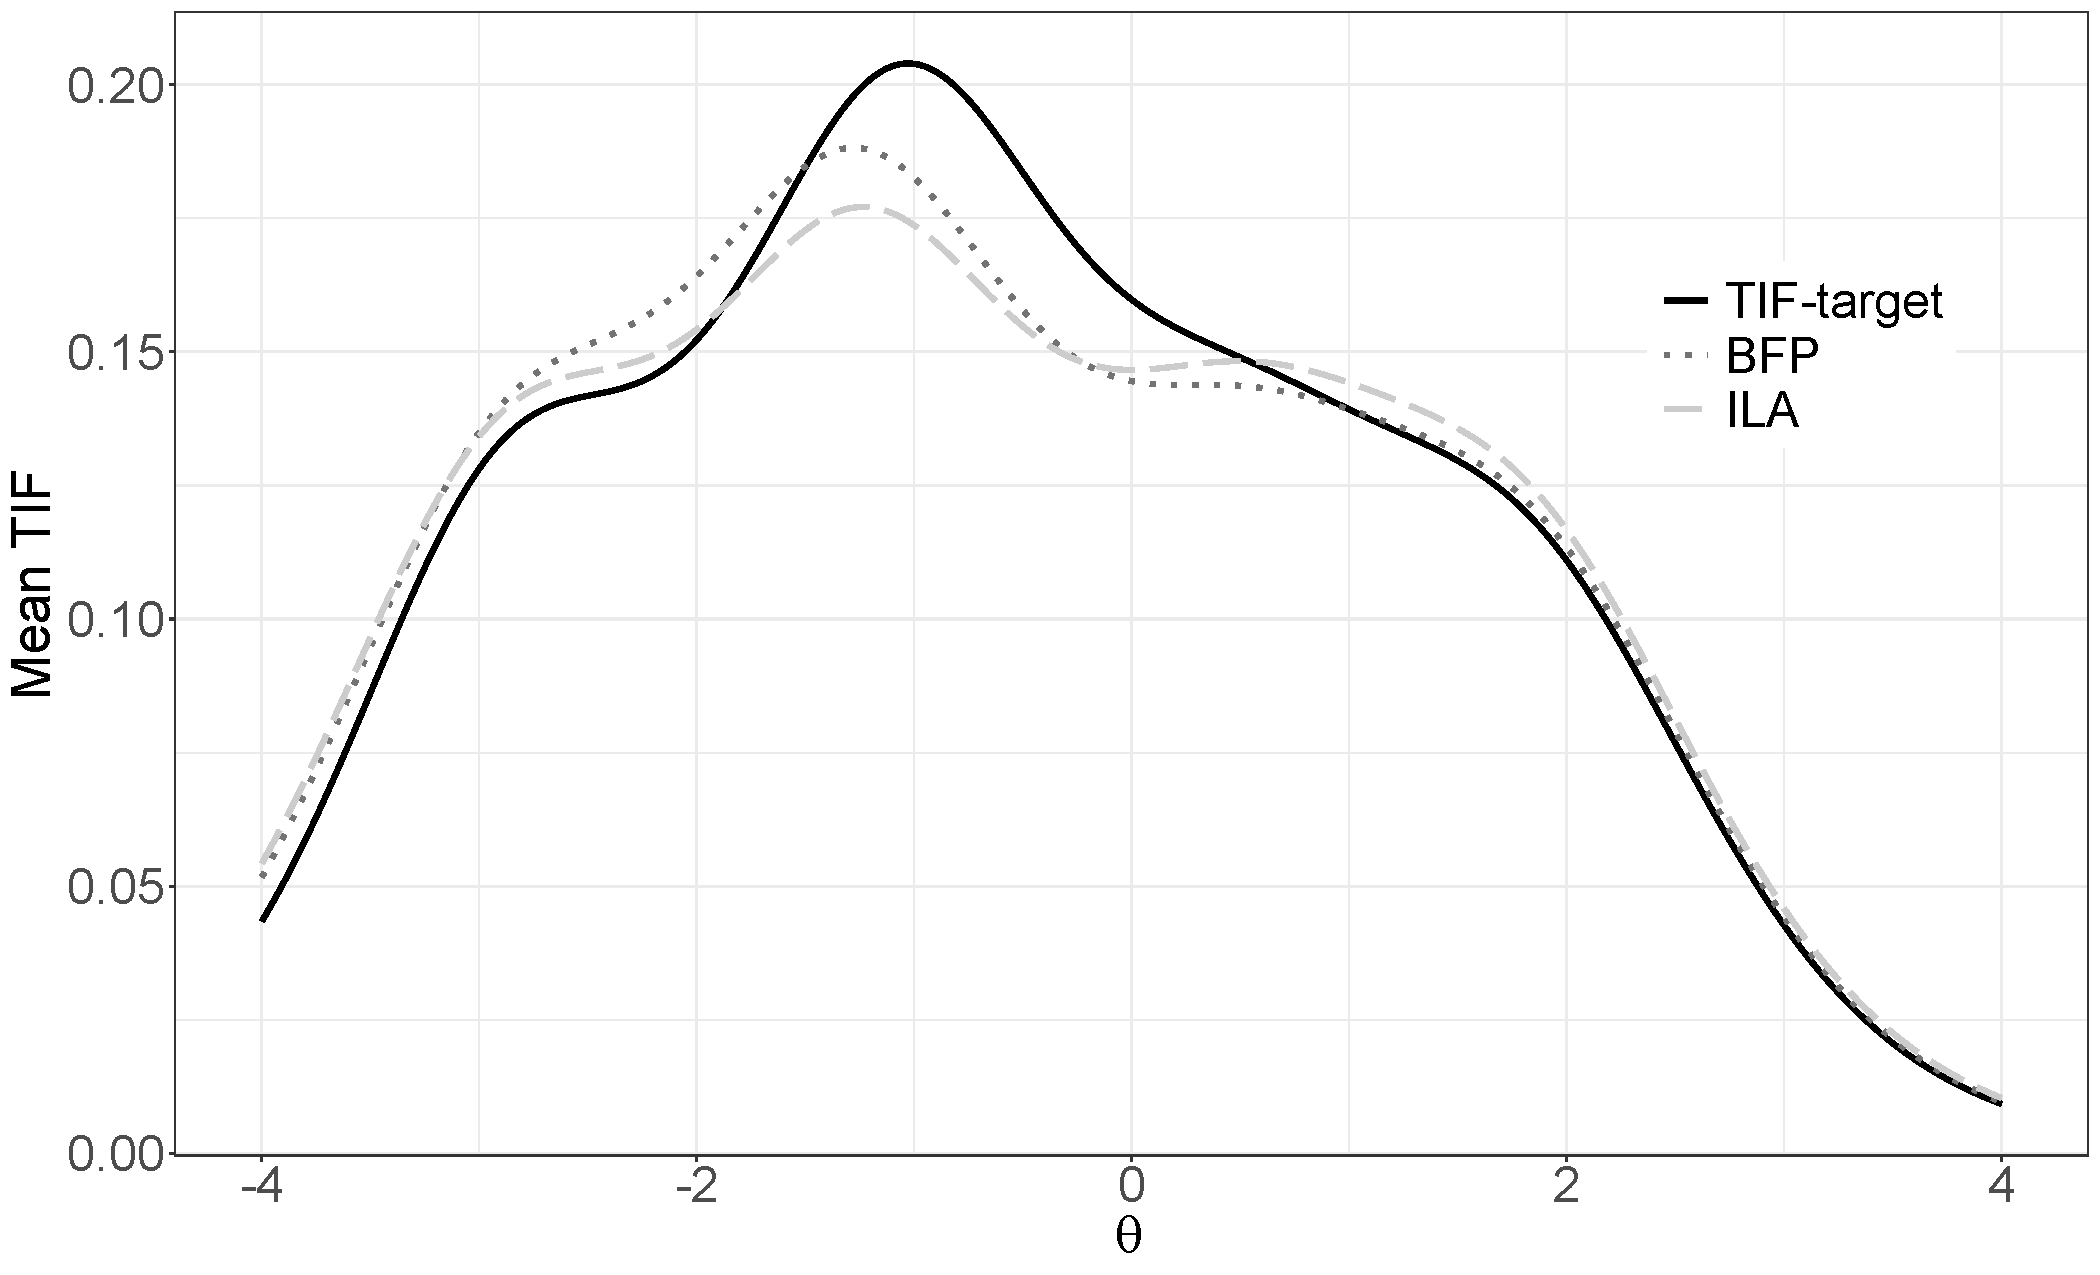
\includegraphics[width=.80\linewidth]{img/equalClose.pdf}	


\centering
\footnotesize{$||Q_{\text{BFP}}|| < ||Q_{\text{ILA}}||$}
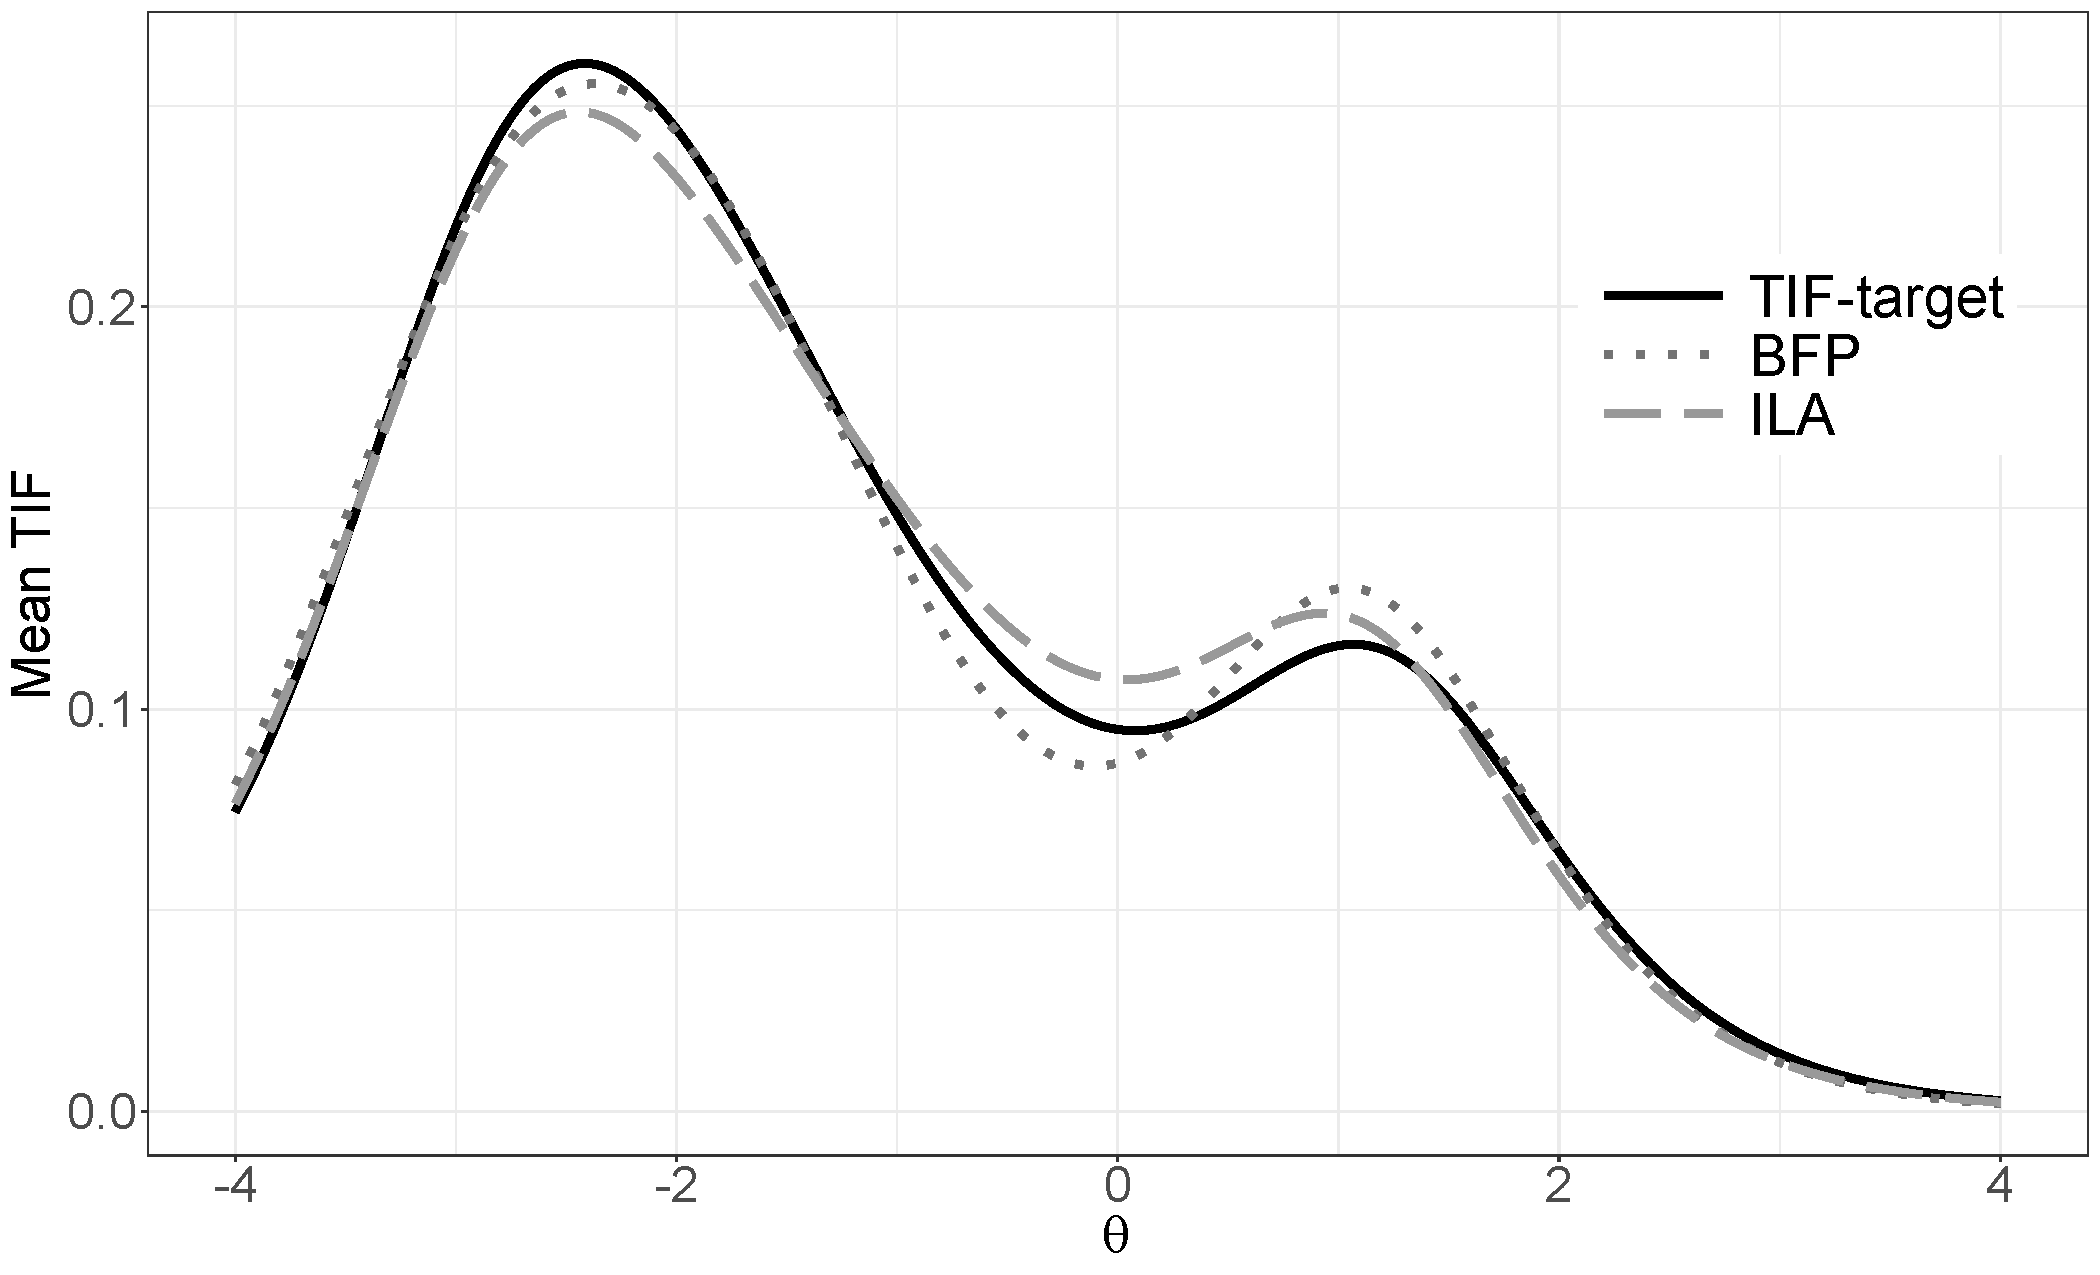
\includegraphics[width=.80\linewidth]{img/moreClose.pdf}	



	\end{column}
	
		\begin{column}{.50\linewidth}
		
		\centering
				\footnotesize{$||Q_{\text{BFP}}|| > ||Q_{\text{ILA}}||$}
		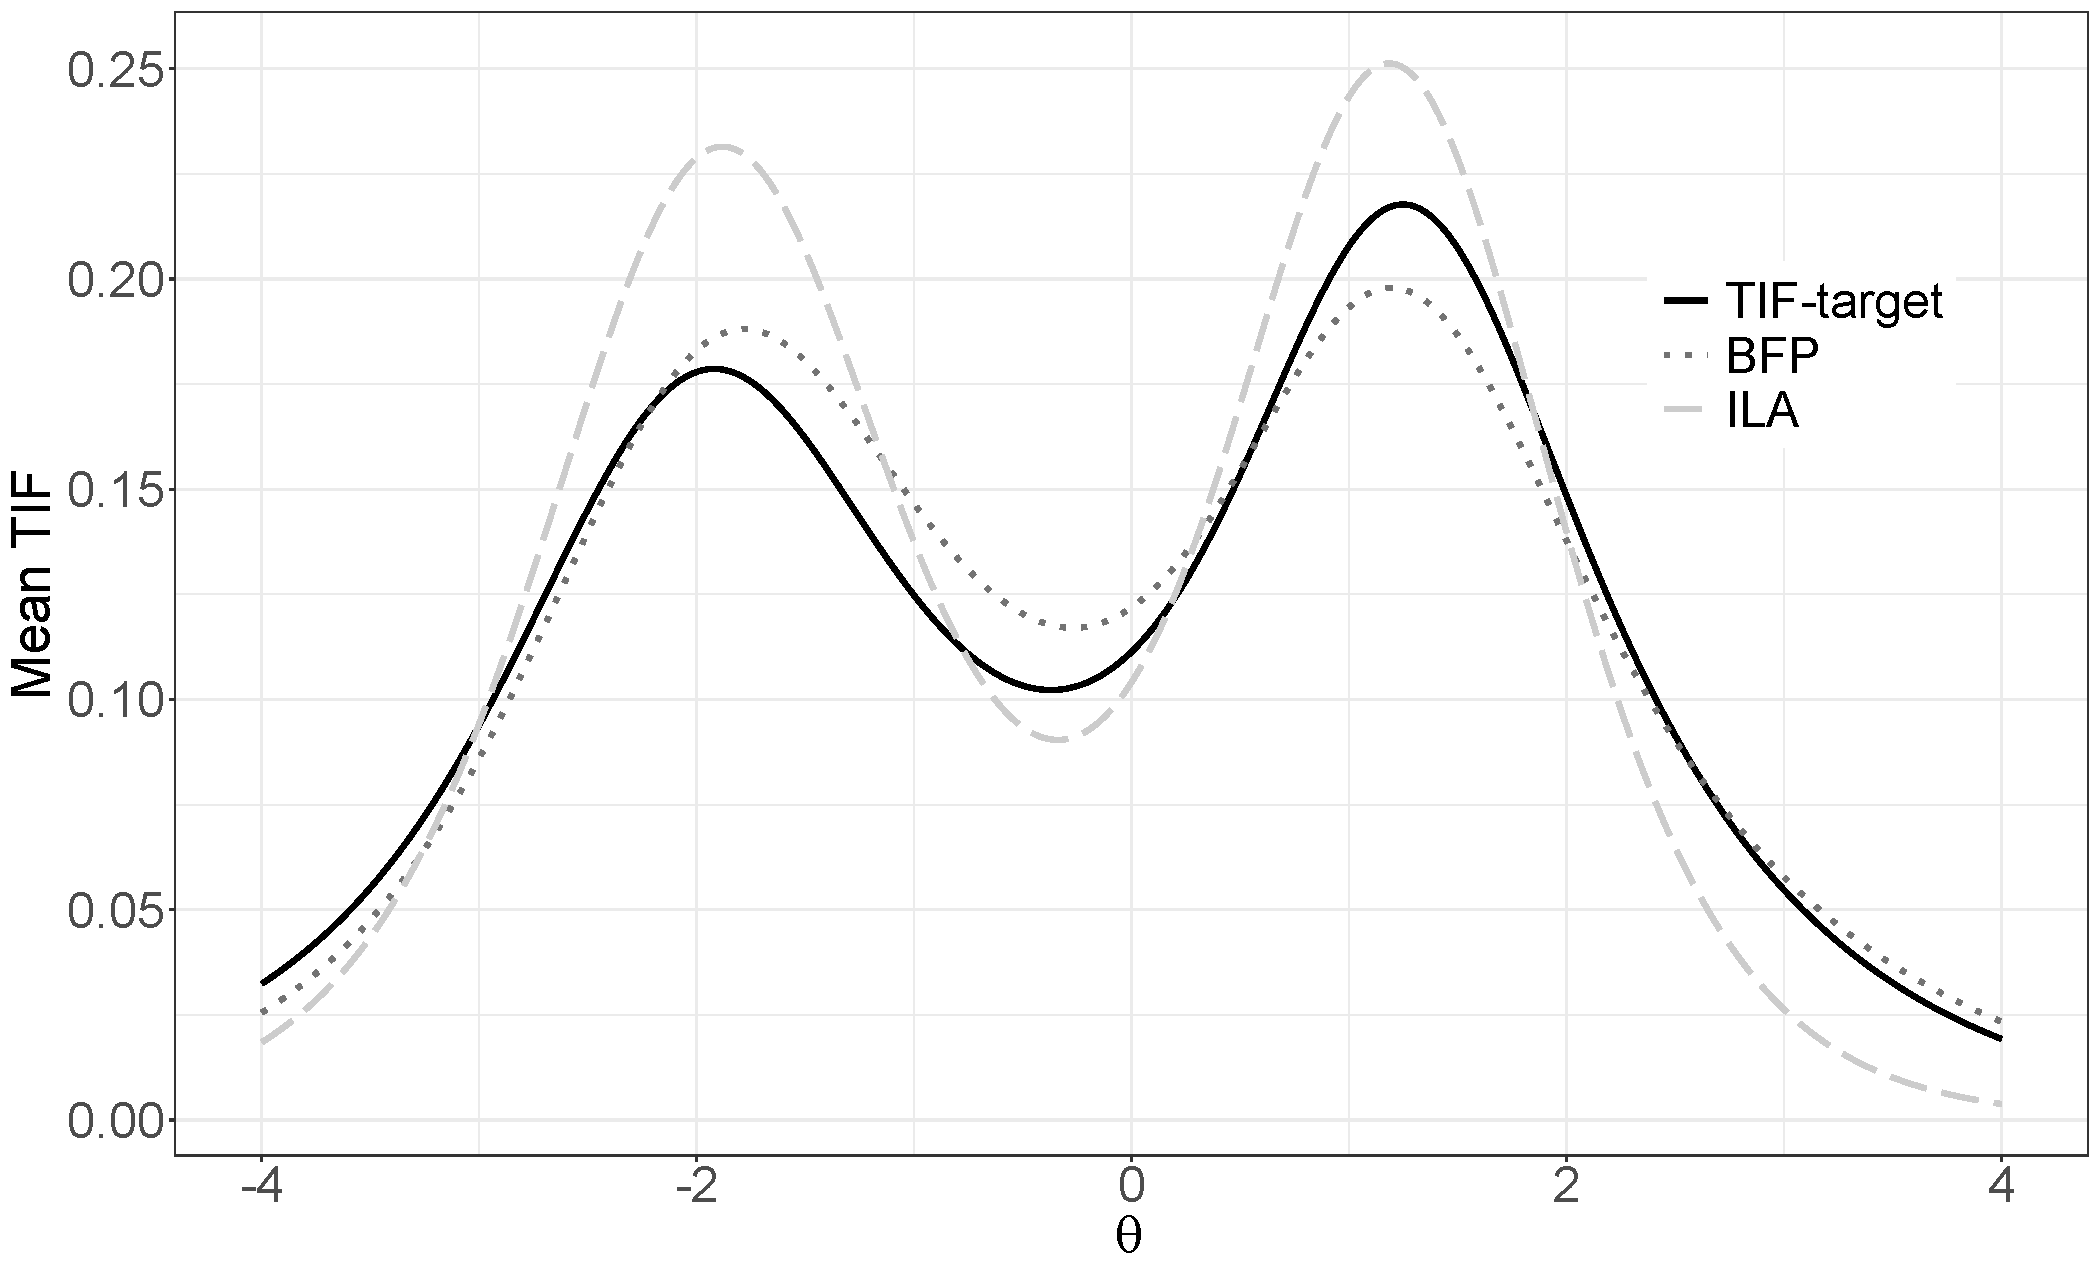
\includegraphics[width=.80\linewidth]{img/lessClose.pdf}	

		
				\centering
						\footnotesize{$||Q_{\text{BFP}}|| < ||Q_{\text{ILA}}||$}
		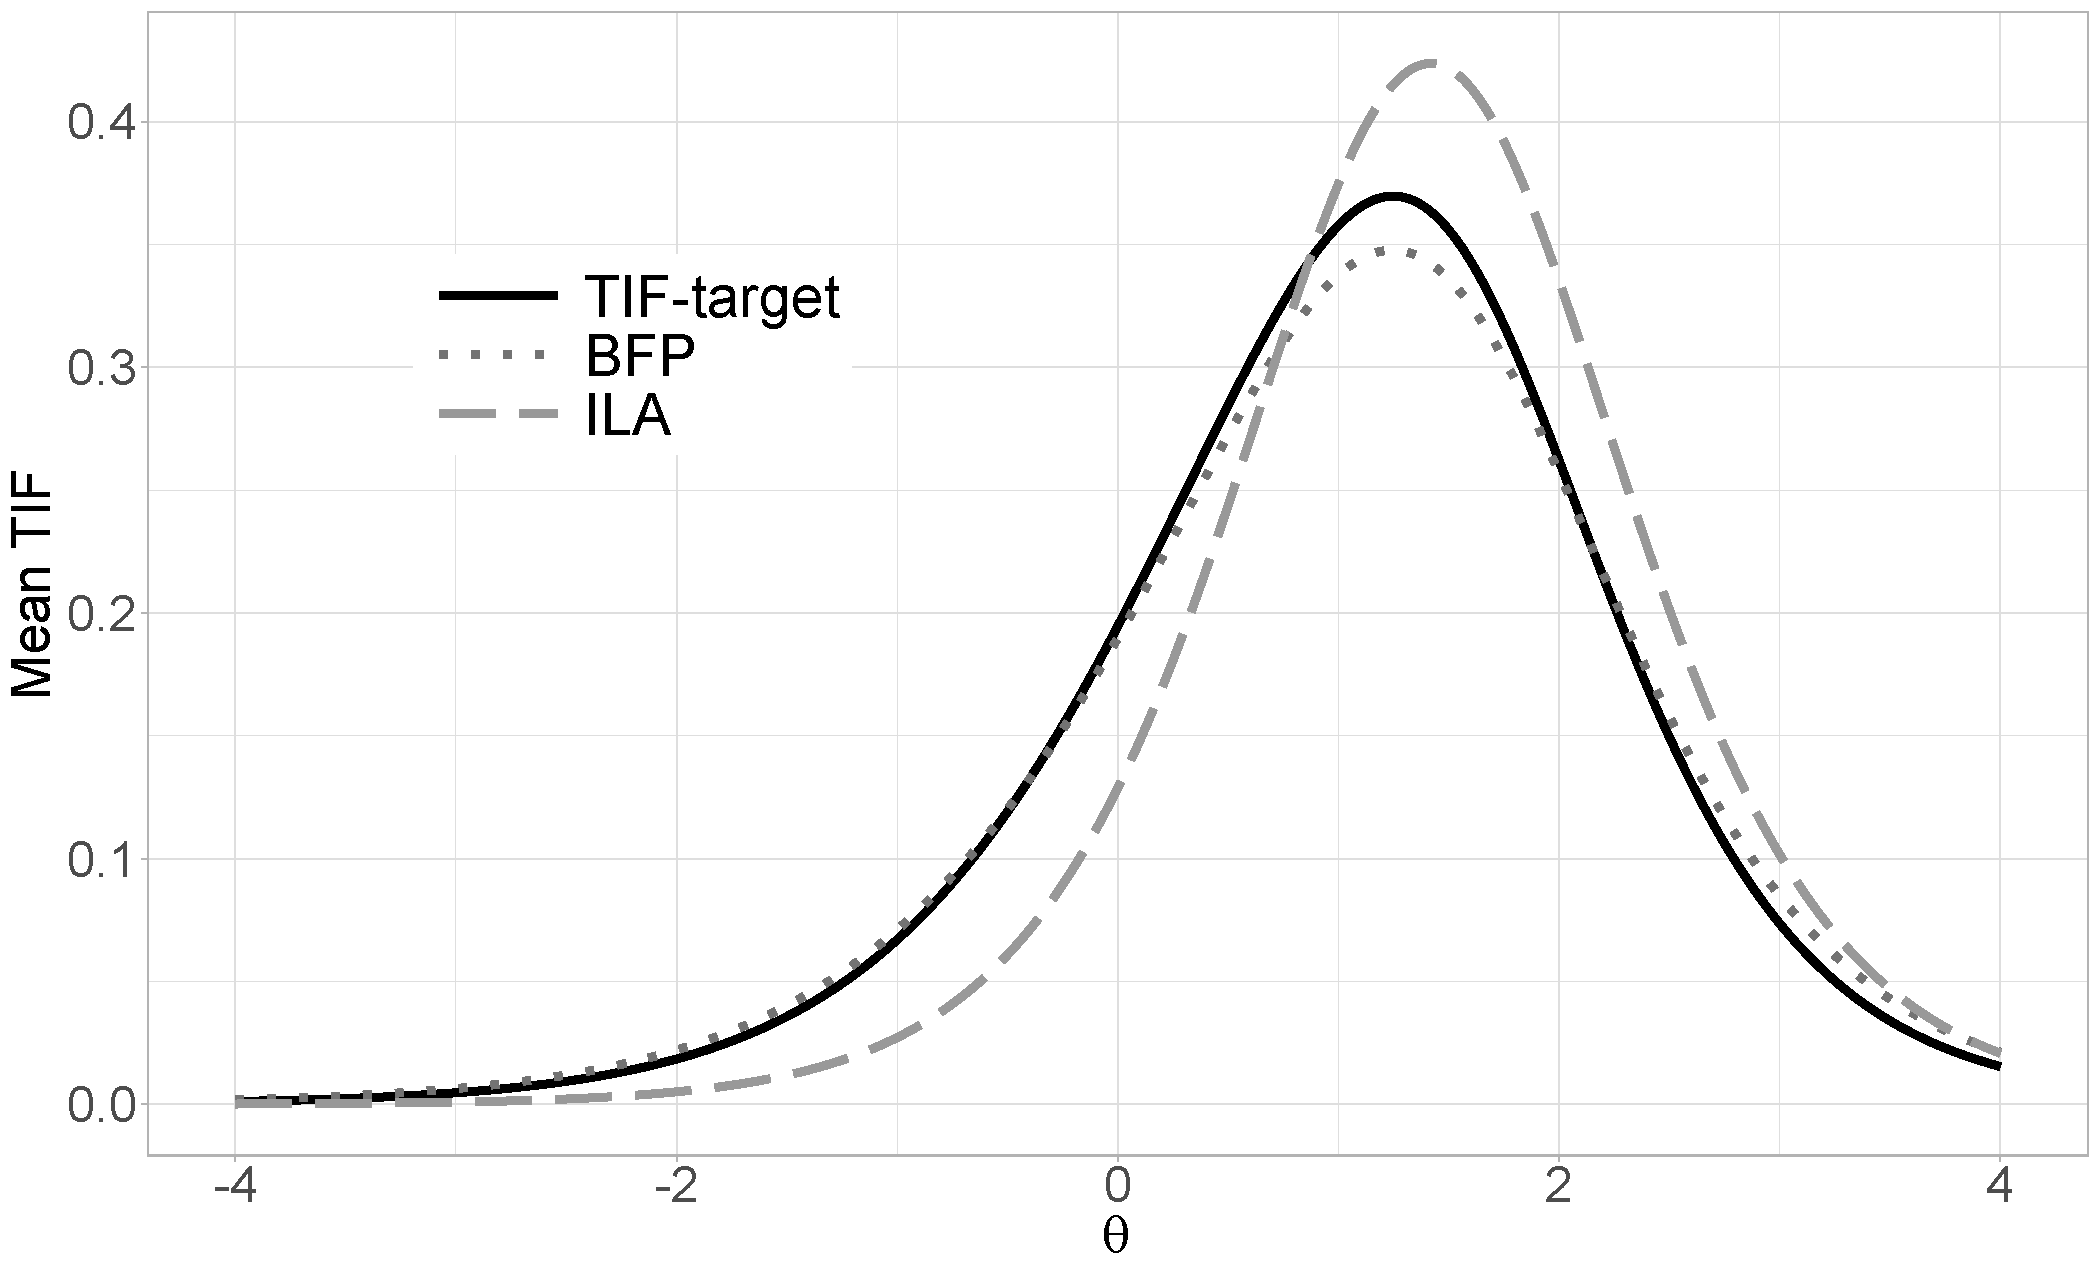
\includegraphics[width=.80\linewidth]{img/lessFar.pdf}	

		
	\end{column}
	\end{columns}
	

\end{frame}



\end{document}
